% Created 2018-02-03 土 00:03
% Intended LaTeX compiler: pdflatex
\documentclass{scrartcl}
    \usepackage{amsmath, amssymb, bm}
		\usepackage[utf8]{inputenc}
		\usepackage[dvipdfmx]{graphicx}
		\usepackage[dvipdfmx]{color}
		\usepackage[backend=biber,bibencoding=utf8]{biblatex}
		\usepackage{url}
		\usepackage{indentfirst}
		\usepackage[normalem]{ulem}
		\usepackage{longtable}
		\usepackage{minted}
		\usepackage{fancyvrb}
    \usepackage[dvipdfmx,colorlinks=false,pdfborder={0 0 0}]{hyperref}
    \usepackage{pxjahyper}
    \usepackage{caption}
		\usepackage{biblatex}
\addbibresource{reference.bib}
\author{筑波大学情報学群情報科学類(201611350) 江畑 拓哉}
\date{\today}
\title{情報特別演習最終レポート}
\begin{document}

\maketitle
\tableofcontents



\section{概要}
\label{sec:org3f45b9e}
今情報特別演習において私は、機械学習を初学者が学ぶための Web アプリ開発を行った。当初は大規模データベースを用いた機械学習APIを作るという目標であったが、特に機械学習を学んでいくにあたり、これの中身を理解するための初学者向けの解説の供給が少ないと感じたため、開発目標をやや変更した。\(\newline\)\\
 今回学習した内容は、 \textcircled{\scriptsize1} 大規模データベースの、特に時系列データベースの比較とその利用法 \textcircled{\scriptsize2} 機械学習等を実装する際に重要となる高速計算を JVM 言語内で行う手法 \textcircled{\scriptsize3} 代表的な時系列分析の一つである(S)ARIMA モデル \textcircled{\scriptsize4} 開発言語として取り上げた Clojure/ClojureScript の、言語自体・これを用いたWeb開発手法、の4分野である。\\
 結果として 時系列データベースとして OpenTSDB を採用し ARIMA モデルとそれに付随する ADF 検定などを実装・解説を作成した。更に JVM 上で高速計算を行うために、\(\href{http://jblas.org/}{jblas}\) や \(\href{https://software.intel.com/en-us/mkl}{Intel \textsuperscript{\textregistered} MATH \ KERNEL \  LIBRARY}\) を用いた GPU 演算 、 OpenCL の利用例を調べ比較し、一部を Web アプリの実装に活用した。そして \(\href{https://clojure.org/}{Clojure}\) という言語を身に着け、Clojure/ClojureScript を用いて JavaScript のライブラリである \(\href{https://reactjs.org/}{React.js}\) などを利用する手法についてまとめ、これらを利用してWebアプリの概形を実装した。\\
\section{序論}
\label{sec:org5f5b576}
この情報特別演習の初期テーマの決定はグループメンバーからの提案が元であった。その概要は、大規模データベースである \(\href{https://hbase.apache.org/}{Apache \  HBase \textsuperscript{\texttrademark}}\) (以降 ``HBase'' と呼称する) を用いて入力されたデータの因果関係を分析、予測する機械学習APIを作成するというものである。ここから因果関係と相関関係の違いについて学習し、機械学習手法について吟味した結果、ニューラルネットを用いた学習手法と、(S)ARIMA モデルを用いた時系列データ予測と Random Forest を用いた欠損値補完を組み合わせたものの2つの手法が議題に上がったが、後者を選択することになりこれを研究することになった。その中で機械学習を学ぶ際にその内部を知る必要があり、学んでいく際にその資料の供給が少ないことを感じ、その資料も兼ね備えたいと考え、また機械学習結果を視覚的にわかりやすく伝える目的も合わせて、Webアプリという形で開発を行うことに目標を定めた。\\
\newline\\
 機械学習という名前は世間に流布しており、それを用いたAPIとして例えば Microsoft Azure の \(\href{https://azure.microsoft.com/ja-jp/services/cognitive-services/computer-vision/}{Computer Vision API}\) 等を上げることができるが、この中身が解説されることはその必要性や機密性の問題から非常に少ない。またPythonやRといった言語やそのライブラリ等に付属している統計処理、機械学習の関数などもその殆どが簡便化されており、例えば \(\href{https://www.rdocumentation.org/packages/forecast/versions/8.1/topics/auto.arima}{auto.arima()}\) 関数などはその中身に踏み込むことなく実行、モデルの比較を行うことができる。これは機械学習の利用者という立場からすれば素晴らしい進歩であると考えられるが、その反面機械学習を学ぶ立場になった場合、その中身を知らない状態でAPIや関数を利用することができるため、手放しに機械学習を理解できたと誤解してしまう可能性がある。\\
 このため主要な機械学習についてその中身を学習できるツールの作成は、統計や機械学習を学びたいと志している、或いは先述のようなツールの中身について興味を持った者に対して、一定の需要があるのではないかと考えている。\\

\section{時系列データベースの比較と OpenTSDB の利用法}
\label{sec:orgb8a7fe0}
一般的に時系列データのような、単調増加する要素を持つデータを通常の大規模データベースに保存することはデータの分散という点から問題が発生する。 \cite{hbase-reference} このため時系列データを扱うためのデータベースを考える必要がある。幸いなことに、初期案にあった HBase に対して時系列データを扱うことができるように拡張した \(\href{http://opentsdb.net/}{OpenTSDB}\) というデータベースがある。OpenTSDB は HTTP API として操作が許されており、また保存されているデータを確認することが容易であるように設計されている。今回は HBase を完全分散モードで利用する、というチームメンバーの目標に沿ってこちらのデータベースを採用した。\\
 他の時系列データベースの提案として考えられるものに、\textcircled{\scriptsize 1} \(\href{https://www.influxdata.com/}{InfluxDB}\) 、\textcircled{\scriptsize 2} \(\href{https://graphiteapp.org/}{Graphite}\) 、 \textcircled{\scriptsize 3} \(\href{https://www.datomic.com/}{Datomic}\) などを挙げることができる。\\
 この章ではそれぞれのデータベースの特徴と利用法を簡潔にまとめる。\\
\subsection{InfluxDB}
\label{sec:org72c7b77}
InfluxDB は InfluxData が開発を行っているデータベースであり、高機能なクラウドシステムを有料で使うことができるほか、オープンソースソフトウェアとしての利用も可能である。このデータベースの利点の一つに、利用方法が簡単であることが挙げられる。シングルノードでの利用に関してのみに焦点を絞れば、2017年12月において \(\href{https://www.archlinux.org/}{Arch\ Linux}\) でのインストールは、パッケージのインストールとサービスの起動の \href{https://wiki.archlinux.jp/index.php/InfluxDB}{2つのコマンド} で利用可能になる。またデータベースの読み書きに関しては、SQLに近い記法を用いた HTTP API を用いて行うことができ、今回の演習における開発言語である Clojure で必要な部分に関するラッパーを書くことは非常に簡単であった。また TICK stack と呼ばれる InfluxDB を含む時系列データを扱うための環境を追加でセットアップすればデータのモニタリング、収集、リアルタイム処理をより効率的に行うことができる。本演習の初期目標ではデータの入力をユーザが行うことができる設定になっていたため、悪意あるデータを監視することが容易であるという点、データベースの外側の分野までの広いサポート環境があるという点からこのデータベースは非常に魅力的である。\\
 このデータベースが扱うデータモデルの概要を以下に示す。\\
\begin{table}[htbp]
\caption{InfluxDB data model}
\centering
\begin{tabular}{|c|c|c|}
\hline
name(required) &  & \\
\hline
\hline
timestamp (required) & fields (required) & tags (optional)\\
\hline
 &  & \\
\vdots & \vdots & \vdots\\
\hline
\end{tabular}
\end{table}

 それぞれの用語についてその意味と例を挙げると以下のようになる。\\
\begin{itemize}
\item name データの名前 (ex. 日経平均株価)\\
 データの名前であり、何に関してのデータであるかを表す。\\
\item timestamp 時刻データ (ex. 2018-01-27T00:00:00Z)\\
 時刻データであり、いつのデータであるのかを示す。この場合の ``いつのデータ'' とは、データの登録日時ではなく、そのデータの発生日時である。\\
\item fields 測定値群 (ex. (終値:12000) (始値:11000))\\
 そのデータが持つ値を示す。いくつかの属性に従って複数の値を格納することができるが、ここに登録されるデータは索引付けされるべきものではないという点でタグ群と意味が異なる。\\
\item tags タグ群 (ex. (記録者:A) (ソース:東京株式市場))\\
 そのデータの持つ属性や追加情報を示す。ここに登録されるデータは索引付けさており、データの絞り込みを行う目的に用いられる。\\
\end{itemize}

\subsection{Graphite}
\label{sec:org6e807ec}
Graphite は Python を中心にして書かれた時系列データベースであり、同じく Python の Webフレームワークである Django と組み合わせることが、 Graphite 自身の Web UI コンポーネントが Django であるという点から、非常に容易である。同時に Python は機械学習に関する API・ライブラリ が豊富に存在しているため、本演習が純粋に ``Web APIの作成'' のみの目標であったならば当然こちらを用いて開発を行っていただろう。またデータベースの導入自体も、 Python のパッケージ管理システムである pip を用いて行うことができることから、純粋に Python のみによってすべてを解決することができる。更に Graphite のドキュメントは豊富に存在しており、例えば Monitoring with Graphite \cite{graphite-oreilly} を挙げることができる。\\
 Graphite の内部について簡単に説明を行うと、主に4つのコンポーネント、Carbon、Whisper、Cario、Djangoを中心に展開する。\\
\begin{itemize}
\item Carbon は、後述するデータベースそのものと言える Whisper にデータを登録する役割を担っており、メトリクス\footnote[1]{metrics: 入手したデータを分析して数値化したもの}のバッファリングを行ったり他のデータベースにメトリクスをリレーさせたりすることができる。\\
\item Whisper は、入手したデータをファイルシステムに書き込み・読み出しを行う役割を担っており、この部分は Ceres と呼ばれるコンポーネントに置き換えることができる。両者の違いは、Whisper が保存領域を固定サイズとして確保するのに対して、Ceres は任意のサイズで保存領域を確保できるということにある。\\
\item Cario は、Graphite のグラフィックエンジンを担当しており、保存されているデータを視覚化する上で非常に重要な役割を果たしている。\\
\item Django は、Cario によって出力されたデータを表示する役割を担っており、データを扱う開発者はこの部分を見てデータを確認することになる。\\
\end{itemize}

 このデータベースが扱うデータモデルは階層構造を取っており、一例を紹介すると以下のようになる。\\
\begin{verse}
``stock\_price.nikkei\_index.close\_price 12000 1517055464''\\
\end{verse}

 上の文字列を送信することによって、 stock\_price の中の nikkei\_index の中にある close\_price という階層に 12000 という値を Unix 時間である 1517055464 のデータとして登録している。つまりこのデータは以下のようにな形に保存されたと考える。\\

\begin{figure}[htbp]
\centering
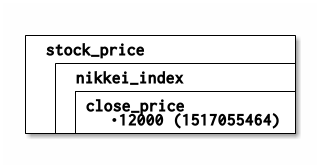
\includegraphics[width=8cm]{hoge.png}
\caption{Graphite example}
\end{figure}

\subsection{Datomic}
\label{sec:orgef40ef0}
 Datomic は他のデータベースとはかけ離れた設計が行われた新しい世代の分散型データベースである。 Clojure の作者である Rich Hickey 氏らが作成し、有料でメンテナンスとアップデートが付属されたクラウドシステムを使うことができる。また一年に限っては無料でこの機能を利用することもできる。これとは別に存在する無料版に関しては分散できるピア数などの制限がかかる。\\
  Datomic には2つの目標「情報を時間によって紐付け蓄積する」 「データベースアプリケーションのモデルをリモートアクセスするものからそれぞれのプログラムの中にあるものとする」\footnote{http://endot.org/notes/2014-01-10-using-datomic-with-riak/} がある。この考え方によって得られた大きな2つの特徴に、\textcircled{\scriptsize 1} Append-Only \textcircled{\scriptsize 2}データベースに独立したクエリーエンジンがある。\\
 Append-Onlyとはその名の通り、追加のみという意味で言い換えれば変更ができないということを意味する。これは情報を時間に紐付けることによって最新の情報を見ることができるため、情報を``書き換える''必要がなくなったためにできたことであり、トランザクション処理などのデータの管理を容易にすることができる。\\
 データベースに独立したクエリーエンジンとは、アプリケーション側でトランザクションやクエリ処理を実行するという意味を示しており、データベースに HTTP API などを用いてクエリを投げデータベース側がそのクエリを処理して結果を送信していたものをアプリケーション側に移す、ということになる。その意味で Datomic はアプリケーション側をピア \footnote{peer} と呼称する。\\
 ピアが扱うデータはデータベースではなくピア側のキャッシュに Read Only な形で LRU \footnote{Least Reacently Use}形式で保持される。データベースは書き込まれたデータを保存し、更新があればそれぞれのピアが持っている、データベースに対して常に開いているノードに告知し、アプリケーション側から要求されるデータ群をそのまま返すことになる。これによってピア側のメモリキャッシュを疑似データベースとして貪欲に使うことができ、データベースのボトルネックを解消することができるようになっている。更にピア側のキャッシュ上のデータベースは実質ゼロコストで用いることができるため、 LRU が最適であるような目的のアプリケーションにこのデータベースを適用した場合、データへのアクセスという点において他のデータベースに性能で劣ることはない。またクエリ処理を分散しているため、多くのクエリ処理をこなさなければならないピアが増えたとしても、キャッシュ上のデータを使っている限りはその処理によってデータベースに負荷がかかることもない。またデータベースの更新をピアに告知しなければならないという点でデータベースへの書き込みがネックになる可能性もあるが、これは論理的に分かれているデータごとにデータベースそのものを分割することで解決することができる。\\
 データベースのアクセス方法は Datalog と呼ばれる Clojure らしいシステムによって扱われるため、SQLに慣れている場合には苦労する可能性があるが、アプリケーションに柔軟に組み込むことができる。これはデータがキャッシュ上に Read-Only な形で存在しているという特性と、 Clojrue が関数型言語の側面を持っているという点を考えれば、データベース上のデータを手元にあるデータであるかのように利用することができるということを意味している。また保存しているデータは必ず Datom という最小単位に分割されており、これを元にして様々な形にデータを変形させることができる。\\
 このデータベースが扱うデータ例を以下に示す。\\

\begin{verse}
\{:nikkei-index/type ``close-price''\\
\hspace*{1em}:nikkei-index/value 12000\\
\hspace*{1em}:nikkei-index/timestamp 1517055464\}\\
\end{verse}
 データは nikkei-index/type に対する値として ``close-price'' が格納されている。nikkei-index に ``close-price'' が含まれているわけではない。\\

\begin{table}{h}
\caption{Datomicの特徴}
\centering
\begin{tabular}{|c|l|}
\hline
目指すもの & \(\cdot\) 情報は時間によって紐付ける\\
 & \(\cdot\) データベースアプリケーションのモデルをそれぞれのプログラム内に移動する\\
\hline
大きな特徴 & \(\cdot\) Append-Only データベース\\
 & \(\cdot\) データベース側ではなくアプリケーション側にクエリ処理エンジンがある\\
\hline
\end{tabular}
\end{table}

\begin{figure}[htbp]
\centering
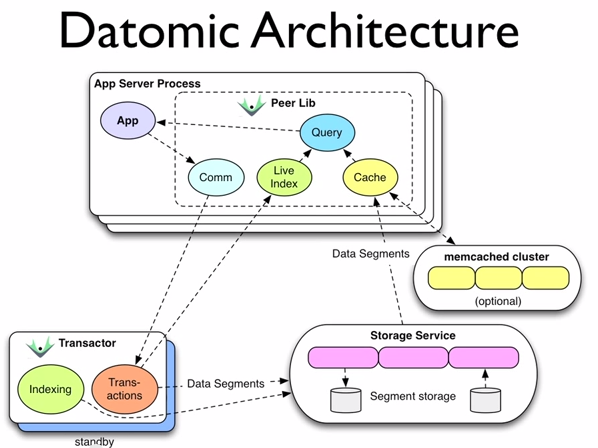
\includegraphics[width=15cm]{./datomic.png}
\caption{\href{http://endot.org/notes/2014-01-10-using-datomic-with-riak/datomic.png}{Talk Notes: Using Datomic With Riakより}}
\end{figure}

\newpage
\subsection{OpenTSDB}
\label{sec:org2699ed7}
OpenTSDB の特徴の説明、セットアップや利用方法に関して説明を行う前に、その基盤である HBase とその周辺知識について簡単にまとめ、その後 OpenTSDB についての説明を行う。\\

\subsubsection{HBase とその周辺知識}
\label{sec:orga926302}
HBase とは \(\href{http://hadoop.apache.org/}{Apache \textsuperscript{\texttrademark} Hadoop \textsuperscript{\textregistered}}\) (以降 ``Hadoop'' と呼称する) と呼ばれる、大規模データの分散処理フレームワークのためのデータベースである。そして Hadoop の分散サービスを形成するために \(\href{http://zookeeper.apache.org/}{Apache \ Zookeeper \textsuperscript{\texttrademark}}\) (以降 ``Zookeeper'' と呼称する)という管理ツールが使われる。\\
\subsubsection{HBase}
\label{sec:org7d5560b}
HBase は NoSQL の一つである。NoSQL は大別して、\textcircled{\scriptsize 1}キーバリュー型\textcircled{\scriptsize 2}ワイドカラム型\textcircled{\scriptsize 3}ドキュメント型\textcircled{\scriptsize 4}グラフ型、があり HBase はワイドカラム型\footnote{簡単に説明するとデータを行ごとではなく列に対して管理しており特定の列を取り出して処理することに最適化されており、高いパフォーマンスやスケーラビリティを持っている。}に属している。\\

\begin{table}[htbp]
\caption{ワイドカラム型の例 (Name列を取り出すこと等を得意とする)}
\centering
\begin{tabular}{|c|c|c|c|c|}
\hline
ID & Name & Email & Birthday & Authorization\\
\hline
001 & Bob & bob @ foo.com & 1998/01/02 & true\\
002 & John & john @ bar.com & 1987/02/01 & false\\
\vdots & \vdots & \vdots & \vdots & \vdots\\
\hline
\end{tabular}
\end{table}

 Hadoop の HDFS (Hadoop Distributed File System) の補完を担っており、複数台のマシンのディスクを一台のディスクであるかのように扱うことができる。全体のデータは Region という単位で分割されており、これをそれぞれのディスクに1つ以上割り振っていくことで分散を行う。\\
 続いて HBase の論理データモデルについて説明を行う。最上位概念は Namespace と呼ばれるもので、この中には Table と呼ばれるデータを表形式で保持している概念を1個以上含んでいる。 一つ以上の RowKey 、一つ以上の ColumnFamily で構成されている。そして ColumnFamily には一つ以上の ColumnQualifier が存在している。行キーである ColumnQualifier と列キーである RowKey の交差点にはそれぞれ Cell と呼ばれる領域があり、ここにデータが格納されることになる。データは Timestamp とともに保存されており、 Cell にはそのデータが重ねて保存される。つまり Cell には Timestamp に紐付けられたデータが複数存在することになる。また、ワイドカラム型であるという特性上、Table は Rowkey でソートされた状態で保存されることになる。\\
 HBase の物理モデルの Table の構造はキーバリュー形式で保存されている。物理モデルの詳細はデータの分散などの説明も必要となるが、これ以上の内容は本演習で理解することができなかったため説明を省略する。\\

\begin{figure}[htbp]
\centering
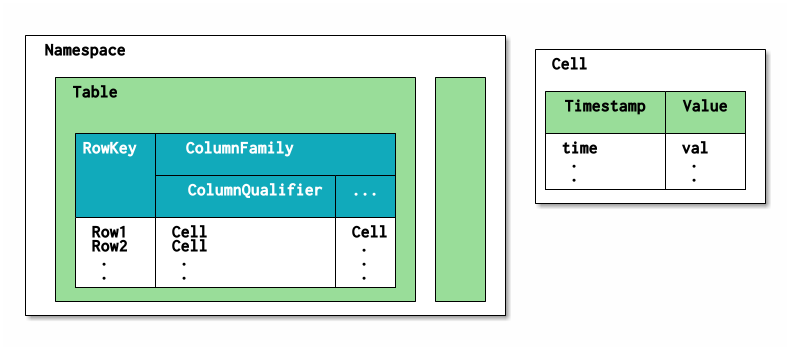
\includegraphics[width=.9\linewidth]{hoge2.png}
\caption{HBase の論理データモデル}
\end{figure}

\subsubsection{Hadoop}
\label{sec:org5f3d256}
Hadoop は大規模データセットの分散処理フレームワークである。 Hadoop はモジュール化されているため、そのコンポーネントの殆どを別のソフトウェアに入れ替えることもできる柔軟な設計がされている。今演習では標準的な Hadoop の構成に付随してインストールされる、\textcircled{\scriptsize 1}Hadoop Common \textcircled{\scriptsize 2}Hadoop YARN\footnote{Yet Another Resource Negotiator} \textcircled{\scriptsize 3}Hadoop MapReduce \textcircled{\scriptsize 4}Hadoop Distributed File System (HDFS) をそのまま利用している。\\
 Common は他のモジュールに利用される基本的なライブラリ群である。 YARN は Hadoop のリソース管理やスケジューリングを行い、 MapReduce は分散処理のためのフレームワークである。 HDFS は分散ファイルシステムで、大容量ファイルを扱うことができる。HDFS は大量の小さなデータを高速に扱うことを不得手としているので、HBase がこの補完を行っている。\\
\subsubsection{Zookeeper}
\label{sec:org340bca3}
Zookeeper は Hadoop などにおける、構成情報の管理、分散処理の提供、またグループサービスの提供なども行う、分散アプリケーション全体を管理するツールである。使用用途は多岐にわたり、例えば Hadoop などにおける構成管理、 \href{http://storm.apache.org/}{Apache Storm}\textsuperscript{\texttrademark} \footnote{リアルタイム高速分散処理フレームワーク} における処理の同期などに用いられる。ツリー状の階層化された名前空間を持ち、ノードと呼ばれる要素にサーバなどを割り当てている。高速処理や高い信頼性があるにもかかわらず、非常に簡単な API を持っていることが特徴である。ベンチマークとしては \href{http://zookeeper.apache.org/doc/current/zookeeperOver.html#fg_zkPerfRW}{Zookeeper\ 3.4\ Documentation} に記載されている。\\


\begin{figure}[htbp]
\centering
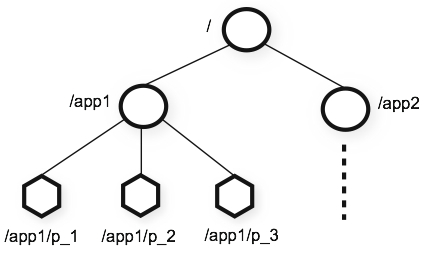
\includegraphics[width=8cm]{./zknamespace.jpg}
\caption{\href{http://zookeeper.apache.org/doc/current/zookeeperOver.html\#fg_zkPerfRW}{Zookeeperの階層構造}}
\end{figure}

\newline\\

\subsubsection{OpenTSDB}
\label{sec:org3a78279}
OpenTSDB とは HBase をホストとした \(\footnote {正確には Google の \href {https://cloud.google.com/bigtable/}{BigTable} もホストとなりうる}\) 時系列データベースで、その構成は\textcircled{\scriptsize 1} 時系列デーモン(以降 TSD と呼称する) \textcircled{\scriptsize 2} コマンドラインユーティリティ、の2つである。特徴としては TSD にマスター・スレーブといった上下関係がないこと、HBase などのホストに各アプリケーションが直接触れる必要がないこと、標準的に保存されているデータをブラウザから視覚的に確認することができることなどが挙げられる。\\
 これによって得られる恩恵として、アプリケーションをチームで開発・維持する際に OpenTSDB を軸にしてデータベース側とアプリケーション側に分割することができるということが考えられる。例えばアプリケーション側はデータベース側の分散等の開発が終わる前に仮設置の HBase に対して OpenTSDB を適用し、アプリケーションをほぼ本環境と同じように動かすことができる。またデータベースの分散数を増やしたい場合は、データベース側にのみ視点を当てて変更を行うことができる。\\

\begin{figure}[htbp]
\centering
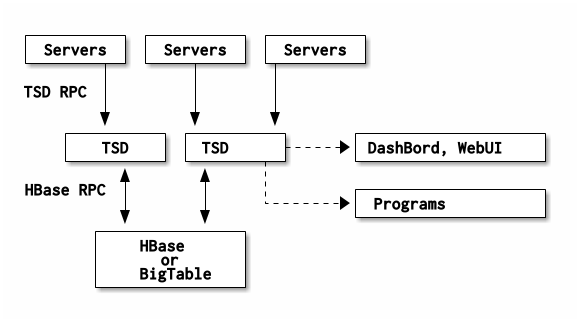
\includegraphics[width=10cm]{hoge3.png}
\caption{OpenTSDB の概略図}
\end{figure}

\newpage\\

 OpenTSDB の論理モデルは Metric と呼ばれるその時系列データのタイトルとも言える概念が最も外側に位置しており、この中にテーブルに近い構造が一つ含まれていると考えることが出来る。このテーブルの行キーはソートされたタイムスタンプであり、時系列データベースの要である。テーブルの列キーはタグと呼ばれるキーバリュー形式の識別子が0以上割り当てられており、これによって欲しいデータの絞り込みを行うことができる。\\

\begin{figure}[htbp]
\centering
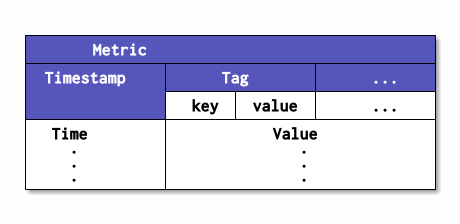
\includegraphics[width=12cm]{hoge4.png}
\caption{OpenTSDB の論理モデル}
\end{figure}

 OpenTSDB はそのアクセスを HTTP API を用いて行うことができる。以降にその概要をまとめる。\\

\subsubsection{OpenTSDB の HTTP API}
\label{sec:org948a86b}
OpenTSDB を利用するにあたって重要な要素に HTTP API の習得がある。このクエリによってアプリケーション開発者はデータの取得や送信を行うことになる。尚、HTTP API を使わずに Telnet を用いる手段もあるが、どちらも機能として同等であるためここでは HTTP API についての説明のみに留める。\\
 API は、データの取得に関してはクエリ文字列とボディ部の両方の手段をサポートしており、ボディ部を用いる場合はクエリ文字列を用いるよりも詳細な検索をかけることが出来る。対してデータの送信は PUT メソッドによるボディ部を用いた手段のみが利用できる。 それぞれの具体例を示すと以下のようになる。\\

\begin{table}[htbp]
\caption{OpenTSDBにおけるクエリ例\textcircled{\scriptsize 1}}
\centering
\begin{tabular}{|c|l|}
\hline
前提条件 & \(\cdot\) http: //localhost:4242 に対して OpenTSDB が開いている\\
クエリ内容 & 1年前から現在までの Metric nikkei-index における\\
 &  タグについてkeyが ``type'' 、valueが ``close-price''\\
 &  であるデータを要求する\\
\hline
クエリ文字列 & \(\cdot\) http: //localhost:4242/api/query $\backslash$\\
 &  ?start=1y-ago\&m=avg:nikkei-index\{type=close\_price\}\\
\hline
ボディコンテンツ & \(\cdot\) http: //localhost:4242/api/query\\
 & \(\cdot\) Content-Type JSON\\
 & \(\cdot\) Body\\
 & \{ "start" : 1y-ago,\\
 &  "queries" :\\
 &   [\{"aggregator" : "sum",\\
 &      "metric" : "nikkei-index",\\
 &       "tags" :\\
 &        \{"type" : "close-price"\}\\
 &  \}]\\
 & \}\\
\hline
\end{tabular}
\end{table}

\begin{table}[htbp]
\caption{OpenTSDBにおけるクエリ例\textcircled{\scriptsize 2}}
\centering
\begin{tabular}{|c|l|}
\hline
前提条件 & \(\cdot\) http: //localhost:4242 に対して OpenTSDB が開いている\\
クエリ内容 & \(\cdot\) Metric ``nikkei-index'' の、\\
 &  タグが、key は``type''、value は``close-price'' である\\
 &  UnixTime が 1517055464 である時間に、\\
 &  12000 という値を保存する\\
\hline
 & \(\cdot\) http: //localhost:4242/api/put\\
 & \(\cdot\) Content-Type JSON\\
 & \(\cdot\) Body\\
 & \{ "metric" : "nikkei-index",\\
 &  "timestamp" : 1717055464,\\
 &  "value" : 12000,\\
 &  "tags" :\\
 &    \{"type" : "close-price"\}\\
 & \}\\
\hline
\end{tabular}
\end{table}

\newpage
\section{Clojure を用いた JVM における高速計算技法}
\label{sec:org0f76e11}
 本演習の開始時、自分のこれまでのプログラム言語学習経歴 \footnote{昨年の情報特別演習においてはPythonを中心に利用し、授業外で Common Lisp をある程度習得した} から、 Lisp の影響を受けた言語を選択することが最も演習に適していると考えており、更に HBase\\
を活用することが決定していたため、 \href{https://www.java.com}{Java} に近い Lisp に近い言語として JVM \footnote{Java virtual machine}上で動作する \href{https://clojure.org}{Clojure} を採用した。また演習を勧めていく上でフロントエンドの開発も行う必要が出てきたため、同様のシンタックスを用いる \href{https://clojurescript.org}{ClojureScript} も採用し、この両方の言語を中心に学習した。\\
  この章ではその内の Clojure における高速計算手法についての学習成果を完結にまとめる。\\

\subsection{Clojure 自身の高速化手法}
\label{sec:org6168cf4}
Clojure に GPU ライブラリ等を適用する以前に純粋な Clojure で最適化されたコードを書くことが高速計算を行う際に重要であることは言うまでもない。本演習では Clojure 自身の学習も兼ね Clojure for the Brave and True \cite{Brave} 、Clojure High Performance Programming \cite{high-performance} を教材に Clojure の最適化手法を学習した。具体的な学習内容としてはプログラム設計の見直しや基本的なシンタックスの見直し、効率の良いスレッド化・並列処理、プログラム全体のパフォーマンス測定法(プロファイリング法)などである。成果としてどこまでの性能向上が認められたかを具体的に比較することは難しいが、性格の良いプログラムを書くことが出来るようになったのではないかと考えている。\\

\subsection{ClojureCL}
\label{sec:org832d004}
\href{http://clojurecl.uncomplicate.org/}{ClojureCL} とは Clojure で OpenCL を用いるためのライブラリで C言語で書かれる OpenCL のコードよりも簡潔なシンタックスで書くことが主張されている。このライブラリはJVM上でOpenCLを動作させるため、 JNI\footnote{Java Native Interface} を基盤としたライブラリである、jocl を用いており、非常に低レベルな部分で OpenCL とリンクしているため、OpenCL そのものの知識が必要となるものの、その速度を十分に体感することが出来る。本演習ではドキュメントに記載されたソースコードを移し、自分の環境においてそれを体験するまでを行った。2018年2月1日においてはより深い理解を行うために、OpenCL in Action \cite{OpenCL} を学習している。\\

\subsection{Neanderthal}
\label{sec:orgdc97458}
\href{http://neanderthal.uncomplicate.org/}{Neanderthal} は、Intel \textsuperscript{\textregistered} MKL を用いた高速行列演算・線形代数のためのライブラリである。その速度はGPUを利用するモードの場合には大規模サイズの行列演算に関しては、 Clojure / Java ライブラリに対しても大凡3000倍の高速化を達成し、CPUを利用する場合においても純粋な Java よりも 100 倍の高速化を達成している。この高速化に関しては後述する Clojure.core.matrix 系ライブラリに対してやや扱いが難しいが、その分大幅な高速化が望むことが出来る。またこのライブラリの依存関係は intel MKL のライブラリ を含むことに意味があるため、 intel MKL のライブラリ \(\footnote{Arch Linuxにおいては /opt/intel/lib,/opt/intel/mkl/lib }\) をアプリケーション内に含んでしまえば標準的な環境で動作させることが出来る。\\

\begin{figure}[htbp]
\centering
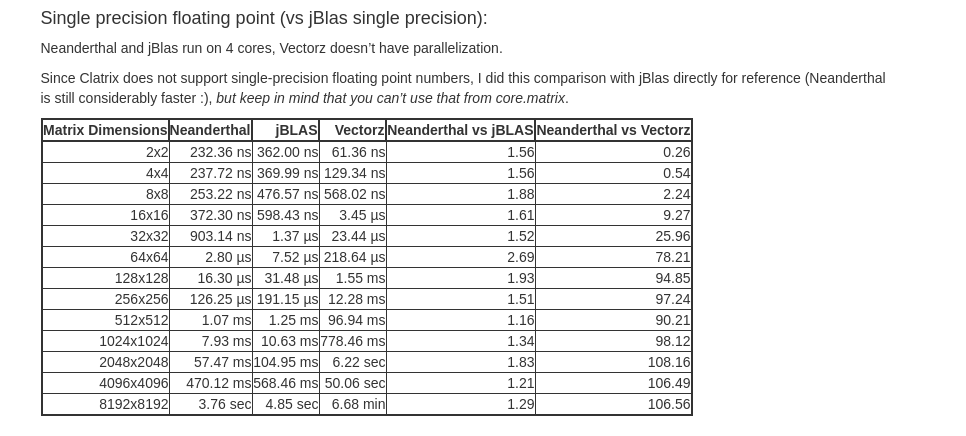
\includegraphics[width=.9\linewidth]{./neanderthal.png}
\caption{ベンチマーク \href{http://neanderthal.uncomplicate.org/articles/benchmarks.html}{Neanderthal Benchmarks} より}
\end{figure}

\newpage
残念ながら本演習では成果物を稼働させるサーバをどのように扱うかについて協議が不足しており、必要とされるライブラリがその環境で入手することが出来るか不明であったため、実装に組み込ませることができなかったものの、実行例の一部をここで紹介することとする。\\

\captionof{listing}{test-Neanderthal.clj}\\
\begin{minted}[frame=lines,linenos=true,obeytabs,tabsize=4]{clojure}
(ns test-neanderthal.core
  (:require
   [uncomplicate.neanderthal.core :refer :all]
   [uncomplicate.neanderthal.native :refer :all]
   [uncomplicate.neanderthal.linalg :refer :all]))

;; ------------------------------------------------------------
;; sample1
(def a (dge 2 3 [1 2 3 4 5 6]))
;; #RealGEMatrix[double, mxn:2x3, layout:column, offset:0]
;;         ↓       ↓       ↓       ┓
;; →       1.00    3.00    5.00
;; →       2.00    4.00    6.00
;; ┗                               ┛

(def b (dge 3 2 [1 3 5 7 9 11]))
;; #RealGEMatrix[double, mxn:3x2, layout:column, offset:0]
;;         ↓       ↓       ┓
;; →       1.00    7.00
;; →       3.00    9.00
;; →       5.00   11.00
;; ┗                       ┛

(mm a b)
;; #RealGEMatrix[double, mxn:2x2, layout:column, offset:0]
;;         ↓       ↓       ┓
;; →      35.00   89.00
;; →      44.00  116.00
;; ┗                       ┛

;; ------------------------------------------------------------
;; sample2
(def A (dge 3 2 [1 0 1 1 1 2]))

(def or (qrfp A))
;; #RealGEMatrix[double, mxn:3x2, layout:column, offset:0]
;;         ↓       ↓       ┓
;; →       1.41    2.12
;; →      -0.00    1.22
;; →      -2.41    3.15
;; ┗                       ┛

(def r (dge 2 2 (:or or)))
;; #RealGEMatrix[double, mxn:2x2, layout:column, offset:0]
;;         ↓       ↓       ┓
;; →       1.41    2.12
;; →      -0.00    1.22
;; ┗                       ┛

(def q (org or))
;; #RealGEMatrix[double, mxn:3x2, layout:column, offset:0]
;;         ↓       ↓       ┓
;; →       0.71   -0.41
;; →       0.00    0.82
;; →       0.71    0.41
;; ┗                       ┛

(def b (dge 3 1 [1 0 -2]))

(def x (mm (tri (trf r)) (trans q) b))
;; #RealGEMatrix[double, mxn:2x1, layout:column, offset:0]
;;         ↓       ┓
;; →       1.00
;; →      -1.00
;; ┗               ┛

;; ------------------------------------------------------------
;; sample2 ~another solution~
(def A (dge 3 2 [1 0 1 1 1 2]))

(def b (dge 3 1 [1 0 -2]))

(def x_ (dge 2 1 (ls A b)))
;; #RealGEMatrix[double, mxn:2x1, layout:column, offset:0]
;;         ↓       ┓
;; →       1.00
;; →      -1.00
;; ┗               ┛
\end{minted}


 5行目までの内容は依存関係の解決である。 Sample1 において単純な行列の足し算を行っており、 Sample2 は QR 分解を用いて \(Ax = b\) の解を求めている。そして Sample2 \textasciitilde{} another solution \textasciitilde{} はこれを存在しているライブラリ関数を用いて解いたものである。両者の速度差はこのサイズの行列演算であればほぼないが、大規模サイズの行列であった場合は後者のほうが圧倒的に速い。後者も前者もほぼ直接 Fortran のライブラリである \href{http://www.netlib.org/lapack/}{LAPACK} \(\footnote{\href{http://www.netlib.org/lapack/}{Linear\ Algebra\ PACKage}}\) を触っているため、計算途中で結果を取り出している前者のほうが効率が悪いためである。\\
 このコードからわかるように、このライブラリが返す値は必ずしも求めている・求まった解答の形を示していない。この理由は Intel MKL 内のソースコードが与えられたデータのメモリに解答を書き込む性質があるためである。この破壊的代入を行う性質は高速化に大きな貢献をしているとともに、高い副作用と難解さを招いている原因であると考えられるが、このライブラリを利用するためには Intel MKL のドキュメントを精読することや、内部の Fortran による実装を眺める他にない。\\

\subsection{Clojure.core.matrix}
\label{sec:org8eb5f7e}
 先に紹介した2つに対してこちらは非常におとなしいライブラリであり、 Clojure の標準的な算術関数のラップや行列演算に関するライブラリの基盤を開発している。ライブラリの基盤というのは、 Java などのオブジェクト指向言語におけるインターフェースのようなもので、実装するべき関数を先に示しておくことで、それを様々な手法によって実装・更新されていくことで長期的にそのライブラリ群を使うことが出来るという利点がある。本演習では、高速さが持ち味である \href{https://github.com/mikera/vectorz-clj}{vectorz-clj} や、 \href{http://jblas.org/}{jblas} を用いて実装されている関数が充実している \href{https://github.com/tel/clatrix}{clatrix} の2つを検討しその両方を利用した。\\

\subsubsection{vectorz-clj}
\label{sec:orgc77e51d}
 Vectorz-clj は純粋に JVM で動作する高速な行列計算ライブラリを掲げており、導入にかかるコストの低さが魅力的である。問題としては行列の結合・切り出しに関する関数のいくつかの挙動が不自然であることで、その点を除いては後述する clatrix よりも概ね高速に動作する。\\
\subsubsection{clatrix}
\label{sec:orgc54e0ea}
 clatrix は jblas をラップしたライブラリであり、行列計算において必要とされる関数をほぼすべて網羅しており、先述のライブラリで不足した部分を補完するために利用した。このライブラリを利用するためには jblas がインストールされていることが必要であるため、標準的な環境にこれを用いたアプリケーションを実行したとしても正常に動作しない。不足する関数を自力で補完することでこのライブラリを使用しないという選択肢もあるため、よりアルゴリズムの能力を磨いて自力で必要な関数を補完したいと考えている。\\

\subsection{ACM3 (Apache Common Math 3)}
\label{sec:org58480db}
 計算速度そのものの向上という意味ではこのカテゴリからはやや離れるが、良質なアルゴリズムによって様々な数学に関するライブラリとして ACM3 がある。本演習ではそのうちの、アメーバ法に関する関数を ARMA モデルにおける係数推定のために利用した。\\
\section{ARIMA モデルによる時系列分析}
\label{sec:org16d20a0}
 (S)ARIMA モデルは時系列分析手法の一つであり、本演習の要とも言える機械学習手法である。本演習ではこのモデルとその周辺手法を実装した。\\
 ARIMA モデルは 正確には ``Autoregressive integrated moving average model'' と呼ばれ、概要は \textcircled{\scriptsize 1} I \textcircled{\scriptsize 2} AR \textcircled{\scriptsize 3} の3要素によって構成されており、この適用できるデータは「非定常過程が見られる」時系列データ \footnote{「定常過程を持っている」時系列データは ARMA (Autoregressive moving average) モデルでの推定となる} である。定常過程と非定常過程の違いについては後述する \ref{sec:org2c869e4} 単位根検定 で説明を行うが、時系列データには非定常過程を持っている場合が少なからずあり、更に ARIMA モデルを ARMA モデルに変換することは非常に容易であるため ARIMA モデルを実装することによって実質的に定常過程、非定常過程両方の性質を持った時系列データを分析することが出来る。また ARIMA モデルの分析対象はある時系列データ内の時点間の関係である、自己相関 \footnote{系列相関ともいう} にある。\\
 また ARIMA モデルの発展として季節階差を削除することを目的とした SARIMA モデルもあるが、こちらは \ref{sec:orga499d69} SARIMA モデルについて にある理由により開発を中断した。\\
 以降にこのモデルの実装において必要になる知識を紹介する。尚ここで使用する式の書式に関しては \ref{sec:org56cd873} 付録に記載する。\\

\subsection{BackShift記法}
\label{sec:orgcadd550}
 BackShift記法とは、記号 ``B'' という演算子を用いた時系列データを表現するための手法であり、以下のような使われ方をする。\cite{otext}
\begin{align}
(1-B)Y_t &=& 1  Y_t - B  Y_t = Y_t - Y_{t-1} \\
(1-B)^2 Y_t &=& (1-B)  (1-B) Y_t \\
(1-B^k) Y_t &=& Y_t - B^k  Y_t \nonumber \\
&=& Y_t - Y_{t-k}
\end{align}
 但し \(Y_t\) は時系列データを表しており、また今後の説明のため、tが大きいほど最近のデータであるものとする。\\
 式(1) は一次階差を表しており、後述する AR モデルでは AR(1) の場合に用いられる。式(2) は二次階差を表しており、同様に AR(2) の場合に用いられる。式(3) はある区間を開けて階差を取っており、これは季節階差を取る際等に用いられる。季節階差という考え方から一旦離れてわかりやすい例を挙げるとすれば、時系列データが月単位のデータであった場合、昨年と今年の差分を取る場合には、 \((1-B^{12})Y_t\) という形をとることになる。\\
 この記法を用いることでn次階差や季節階差を表しやすくなり、また関数型言語などにおいてはその実装の手がかりを得ることが出来る \footnote{$(1-B^n)$という意味を持つ関数を定義することで理論上ARIMAモデルに必要な階差に関する関数は満足することが出来る}。\\

\subsection{単位根検定}
\label{sec:org2c869e4}
 実世界に存在する多くの時系列データは非定常過程を持っていることが示唆されている。この示唆について Jackknifing multiple-window spectra \cite{389899} から有名な一説を引用すると以下のようになる。\\
\begin{verse}
Experience with real-world data, however, soon convinces one that both stationarity and Gaussianity are fairy tales invented for the amusement of undergraduates.\\
\vspace*{1em}
- Thomson, 1994\\
\end{verse}

 ARIMA モデルでは「非定常な」時系列データを「定常な」時系列データに変換した上で ARMA モデルに適用することになる。一般にこの階差は一次であるらしいが、実装側では以降に紹介する ADF検定 をおこなうことで定常性を判定した。またこの他にも、KPSS 検定や Ljung-Box 検定などがあるが、単位根検定という観点から KPSS 検定のみを追加で紹介することとする。\\

 以降における \(y_t\) について定義する。 \(Y_t\) を議論の時系列データとして、\\
\begin{align}
y_t = Y_t - E(Y_t) = Y_t - \mu - \mu_1 t
\end{align}
正確ではないが、ここにおける \(\mu\) は \(t = 0\) における時系列データの値、 \(\mu_t\) は 時系列データの傾きと考えることが出来る。\\

\subsubsection{定常性の性質}
\label{sec:org262d599}
 ここまで``定常性''という言葉を多用してきたが、この定常性について簡単に触れておく。定常性とは同時分布が時間を通じて変わらないこと \footnote{この同時分布が同一であることを持つ時系列過程を特に``強定常である''という} を意味しており、以下のような性質を持っている。\\

\begin{itemize}
\item \(E(Y_t) = \mu\) \\
 母平均 (population mean) は時点 t に依存しない。\\
\item \(Var(Y_t) = \gamma_0\) \\
 分散 (variance) は 時点 t に依存しない\\
\item \(Cov(Y_t, Y_{t-j}) = \gamma_j\) \\
 共分散 (covariance) \footnote\{\$\(\sigma\)\_\{Y\_t Y\_\{t-j\}\}\$と表すこともある\} は 時点 t に依存しない\\
\end{itemize}

 更に \(E(Y_t) = \mu \land Cov(Y_t, Y_{t-j}) = \gamma_j\) のみである場合を特に``弱定常である''という。\\

 逆に非定常過程の時系列データに目を向けたとき、経済学上重要な要素に以下のようなものがある。\\
\begin{itemize}
\item 確定的トレンド (deterministic trend)\\
  \(Y_t = \beta t + \epsilon_t \ where \ \epsilon_t \sim iid(0, \sigma^2)\) と表され、\(E_{DT}(Y_t) = \beta_t\) 、 \(Var_{DT}(Y_t) = \sigma^2\) である。こちらは直ちにトレンド定常 (trend stationarity) という形に変形することが出来る。\\
\item 確率的トレンド (stochastic trend) 又は単位根過程\\
  \((1-B)Y_t = \beta + \epsilon_t \ wherer \ \epsilon_t \sim iid(0,\sigma^2)\) と表され、 \(E_{ST}(Y_t) = \beta_t\) 、 \(Var_{ST}(Y_t) = t \sigma^2\) である。\\
 確定的トレンドに比べこちらは時間が経過する程に大きな影響を及ぼすことになる。こちらは後述する単位根検定として利用できる ADF 検定や KPSS 検定を行うことで発見することが出来る。\\
\item 構造変化\\
 その時系列が予期しない変化(経済データであるならば、例えば突発的な戦争や飢餓)を受けた際に起こる。本来はこれに対する検定も用意するべきであったが、どのような条件をフラグとして検定が行われるべきであるかが理解できなかったため実装することができなかった。\\
\end{itemize}

\begin{figure}[htbp]
\centering
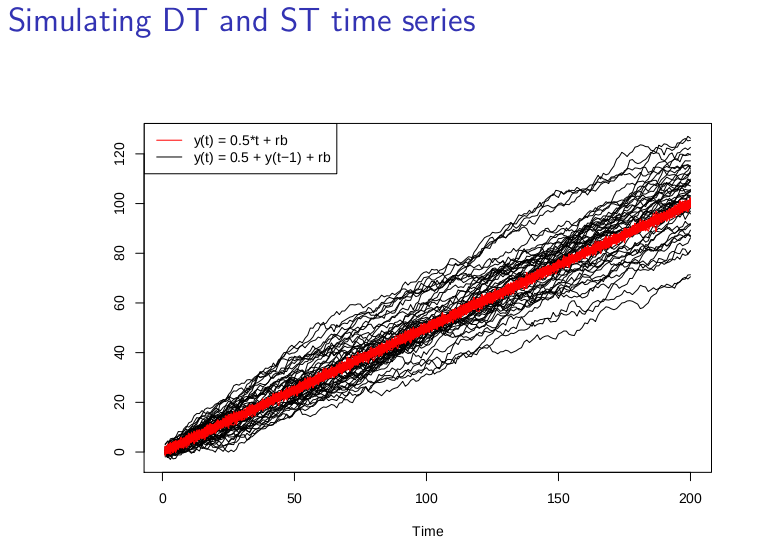
\includegraphics[width=16cm]{./hedibert.png}
\caption{difference between Deterministic and Stochastic trend \cite{hedibert}}
\end{figure}

\newpage\\
\subsubsection{ADF 検定}
\label{sec:orga0e906e}
 ADF 検定 (Augumented Dickey-Fuller test) は DF 検定 (Dickey-Fuller test) の拡張である。\\
 DF 検定とは \(y_t\) について自己回帰モデル AR(1) を作成し以下の条件を用いて仮説検定を行う手法である。\\
 AR(1)モデル \(y_t = \theta y_{t-1} + \epsilon_t \  where \ \epsilon_t \sim iid(0, \sigma^2)\) とする。(AR モデルそのものについては \ref{sec:orgd8b03be} AR モデル で解説を行う)\\
 単位根を持っていることを帰無仮説とし、定常であることを対立仮説であるとする。\\
 つまり、帰無仮説 \(H_0\) と対立仮説 \(H_A\) は以下のように定義できる\\
\begin{align}
H_0\ :\ \theta = 1 \\
H_A\ :\ \theta < 1
\end{align}
 ここからモデルを変形し、以下の式を立てる。\\
\begin{align}
\Delta y_t = (\theta - 1) y_{t-1} + \epsilon_t   
\end{align}
 上式において、\(\pi = (\theta - 1)\) と置換した場合、帰無仮説と対立仮説は以下のように更新される。\\
\begin{align}
H_0\ :\ \pi = 0 \\
H_A\ :\ \pi < 0
\end{align}
 この検定値は簡単な t 検定によって求めることが出来、以下の式によって得られる。\\
    \begin{align}
\widetilde{\tau} &= (\hat{\theta} - 1) / {se(\hat{\theta})} \nonumber \\ 
                 &= \hat{\pi} / se(\hat{\pi})
    \end{align}
 これを自ら指定した有意水準(5\% 又は 1\% であることが多い) において検定する。この検定手法では対立仮説が成り立つならば定常性を認めることが可能である。混乱を招かないために強調するが、この検定における帰無仮説は、``単位根を持っている''ことである。これが棄却されれば``定常である''ことを認めることができる。\\
 また上の場合において、元データの一次階差と取っていることが明らかであるが、この検定で定常であると認められた場合、このデータは 1次の単位根 があるという。同様に d次の単位根がある とは、d - 1 次までの単位根検定においてすべて 非定常である と判断され、 d 次において初めて 定常である と判断されたことを示している。\\
 DF 検定が AR(1) モデルに対する検定であることにたいして、ADF 検定は AR(n) モデルにまで対象を拡大したものであり、一般式は難解であるため省くが、例えば AR(3) モデルは以下のように示すことが出来る。\\
   \begin{align}
   y_t &= \theta_1 y_{t-1} + \theta_2 y_{t-2} + \theta_3  y_{t-3} + \epsilon_t \ where \ \epsilon_t \sim iid(0,\sigma^2) \\
   y_t - y_{t-1} &= (\theta_1 - 1) y_{t-1} + \theta_2  y_{t-2} + \theta_3  y_{t-3} + \epsilon_t \\
   \Delta y_t &= (\theta_1 + \theta_2 + \theta_3 - 1)  y_{t-1} \nonumber \\
&+ (\theta_2 + \theta_3) (y_{t-2} - y_{t-1}) + \theta_3 (y_{t-3} - y_{t-2}) + \epsilon_t \nonumber \\
&= (\theta_1 + \theta_2 + \theta_3 - 1) y_{t-1} + (\theta_2 + \theta_3) * \Delta y_{t-1} + \theta_3 \Delta y_{t-2} + \epsilon_t
   \end{align}
 これより \(\pi = (\theta_1 + \theta_2 + \theta_3 - 1)\) とおいて DF 検定と同様に t 検定を行う。\\
 尚この検定にはいくつかの追加要素として、定常過程にある時系列データの平均値を考えるパターンや、時系列データに傾きがある場合を考慮したパターンがある。これらは人為的にデータを確認することで決定するが、 R 言語や Python などの ADF 検定ではすべてのパターンを一度に実行している場合がある。これは ADF 検定そのものは計算コストが低いため、すべてのパターンを網羅しても問題がないためである。\\
\subsubsection{KPSS 検定}
\label{sec:org0c33a4f}
 KPSS 検定 (Kwiatkowski-Phillips-Schmidt-Shin test) とは先述の ADF 検定に対して帰無仮説と対立仮説を反転させたものとイメージすることが出来る。この検定においては以下の式を中心に展開する。\\
\begin{align}
Y_t &= \xi_t + \epsilon_t \nonumber \\
 &where \ \xi_t = \xi_{t-1} + \upsilon_t \ \upsilon_t \sim iid(0, \sigma_{\upsilon}^2)\  \epsilon_t \sim iid(0, \sigma^2)
\end{align}
 この式における \(\xi_t\) はランダムウォークを示している。尚ランダムウォークとは次に現れる値が確率的にランダムであることを示す。また、\(\epsilon_t\) はその性質から定常過程を示している。\\
 仮に \(\sigma_{\upsilon}^2 = 0\) であるとしたとき、\(\xi_t = \xi_0\) であることから上式に影響を加える要素は \(\epsilon_t\) のみとなり、つまり \(Y_t\) は定常であるとみなすことが出来る。これを用いて上式を変形すると以下のようになる。\\
\begin{align}
Y_t = \hat{\mu} + \hat{\epsilon_t}
\end{align}
 ここで仮説検定を行う。帰無仮説は 定常過程を示している式(15)であり、つまりは式(14) における \(\sigma_{\upsilon}^2 = 0\) である。対立仮説はこの逆であり、非定常であること、つまり \(\sigma_{\upsilon}^2 > 0\) である。\\
\begin{align}
H_0 \ :\ \sigma_{\upsilon}^2 = 0 \\
H_0 \ :\ \sigma_{\upsilon}^2 > 0
\end{align}
 検定は以下の式を用いて行う。\\
\begin{align}
KPSS &= 1/T^2 (\Sigma^{T}_{t = 1}S_t^2)/ \hat{\sigma^2_\infty} \nonumber \\ 
&where\  S_t = \Sigma_{s=1}^t \hat{e_s} 
\end{align}

 また上式における \(\hat{\sigma^2_\infty}\) とは \(\epsilon_t\) の長期変動に関する HAC 推定量 \footnote{特に Newey-West 推定量を用いられることが多い} である。\\
 以下に \(\sigma^2_\infty\) の例を示す。\cite{STAN:STAN272}
\begin{align}
\sigma^2_\infty = \lim_{T \rightarrow \infty} (1/T E((\Sigma_{t=1}^T \epsilon_t)^2))
\end{align}
 ADF 検定あったようにこちらにもいくつかのパターンがあり、トレンド定常の場合などの場合に合わせた形に 式(14) が存在し、それに伴って仮説検定の内容に多少の変化がある。\\
実装においては HAC 推定量を実装することができなかったため、KPSS検定も実装することができなかった。\\
\subsection{AR モデル}
\label{sec:orgd8b03be}
 AR(p) モデル (自己回帰モデル) は以下の式で表すことが出来るモデルである。重回帰モデルが説明変数の線型結合を用いて関心のある変数を予測していること対して、自己回帰モデルは説明変数を過去の観測値に置き換えたものであると言える。\\
\begin{align}
Y_t &= c + \phi_1  Y_{t-1} +\phi Y_{t-2} + \cdots + \phi_p  Y_{t-p} + \epsilon_t \nonumber \\
&= c + \Sigma_{i=1}^{p} (\phi_i  Y_{t-i}) +\epsilon_t  \nonumber \\
&where \  c \ is\  constant \ \nonumber \\ 
&\ \ \ \ \ \ \ \ \ \ \epsilon \sim iid(0, \sigma^2)
\end{align}

\subsection{MA モデル}
\label{sec:org9a90c25}
 MA(q) モデル (移動平均モデル) は以下の式で表すことが出来るモデルである。同様に重回帰モデルの説明変数を過去のノイズの重みに置き換えたものであると言える。これとよく似たものに移動平均という手法があるが、移動平均は過去の値のサイクルを推定するために用いられ、MA(q) モデルは将来の値を予測するために用いられる。\footnote{移動平均とMAモデルは正確には別のものであり、混同されるべきではない。MAモデル自体は有限インパルス応答に近い発想である。cite:2012カルマンフィルタの基礎}\\

\begin{align}
Y_t &= c + \epsilon_t + \theta_1 \epsilon_{t-1} + \theta_2 \epsilon_{t-2} + \cdots + \theta_1 \epsilon_{t-q}   \nonumber \\
&= c + \epsilon_t + \Sigma_{i=1}^{q} (\theta_i \epsilon_{t-i})  \nonumber \\
\end{align}
\subsection{ACF と PACF}
\label{sec:org3273366}
ARMA モデルにおいて\footnote{ACF, PACFは定常過程であるデータに適用される}、AR(p), MA(q) の p, q の値を決定する際の指標となるものに、ACF、PACFがある。この2つはグラフによって視覚化され、この2つのグラフから p, q の値は手動で決定される。\footnote{R言語における auto.arima 関数などはこのような手間なしでモデルを決定することが出来るが、これは p, q などの値を元データにかかわらず適当に複数定めモデルを作成し、AICなどを用いて最も良いモデルを選択しているからである。}\\
\subsubsection{ACF}
\label{sec:org4da0238}
 ACF (autocorrelation function) は自己相関係数とも呼ばれ、元データとある時点分だけずらしたデータとの相関係数を計算する。つまり以下の式を計算することになる。尚、\(t-s\) はそのずらした量(ラグと呼ぶ)である。またこの場合に求まる値を、\(t-s\) 次のACFと呼ぶことがある。\\
\begin{align}
\rho(s,t) &= (E((Y_t - \mu_t)(Y_s-\mu_s)))/(\sigma_{Y_t}\sigma_{Y_s}) \nonumber \\
&= (E((Y_t - \mu_t)(Y_s-\mu_s)))/\sigma^2 \nonumber \\
&= Cov(Y_t, Y_s)/\sigma^2
\end{align}
 上式では \(\sigma_t\sigma_s = \sigma^2\) が成り立っている。これは定常過程を持つ時系列データの分散が時点に依存しないためである。\\
\subsubsection{PACF}
\label{sec:org009c356}
 PACF (partical autocorrelation function) は偏自己相関とも呼ばれ、ある時点とそこからある時点分だけ離れた時点の二点間のみの相関関係である。一般式は複雑であるため、二次、三次の PACF の式を示す。尚、一次の PACF は 一次の ACF に等しい。計算の都合上、k次の PACF を \(\phi(k, k)\) と表す。\\
\begin{align}
\phi(2, 2) &= Cov(Y_t,Y_{t-2}|Y_{t-1})/\sigma_{Y_t|Y_{t-1}}\sigma_{Y_{t-2}|Y_{t-1}}) \\
\phi(3, 3) &= Cov(Y_t,Y_{t-3}|Y_{t-1},Y_{t-2})/(\sigma_{Y_t|Y_{t-1},Y_{t-2}}\sigma_{Y_{t-3}|Y_{t-1},Y_{y-2}})
\end{align}
 このように式がラグごとに異なるため、実装上計算には以下の行列式を用いた Durbin-Levinson recursion が用いられることが多い。以下の式における \(\rho_s\) とは ACF \(\rho(s, t)\) を示している。\\
\begin{align}
\begin{equation}
\left(\begin{array}{ccccc}
\rho(0) & \rho(1) & \rho(2) & \cdots & \rho(k-1) \\
\rho(1) & \rho(0) & \rho(1) & \cdots & \rho(k-2) \\
\rho(2) & \rho(1) & \rho(0) & \cdots & \rho(k-3) \\ 
\vdots  & \vdots  & \vdots  & \ddtos & \vdots \\
\rho(k-1) & \rho(k-2) & \rho(k-3) & \cdots & \rho(0)
\end{array}\right)\left(
\begin{array}{c}
\phi(k, 1) \\
\phi(k, 2) \\
\phi(k, 3) \\
\vdots \\
\phi(k, k) 
\end{array}\right)=\left(\begin{array}{c}
\rho(1) \\
\rho(2) \\
\rho(3) \\
\vdots \\
\rho(k) \end{array}\right)
\end{equation}
\end{align}
\subsubsection{p, q の決定法}
\label{sec:orgbb64aef}
\subsection{係数推定}
\label{sec:org3979c79}
\subsubsection{対数尤度}
\label{sec:org6cb9edd}
\subsubsection{AIC}
\label{sec:org87022d8}
\subsubsection{最小二乗法}
\label{sec:org2e21edf}
\subsubsection{アメーバ法}
\label{sec:org627a832}
\subsection{SARIMA モデルについて}
\label{sec:orga499d69}
\section{Clojure/ClojureScript を用いた Web 開発}
\label{sec:orgf38a223}
\subsection{Clojure によるバックエンド開発}
\label{sec:org3c65324}
\subsubsection{Luminus Framework}
\label{sec:org6596613}
\subsubsection{Swagger UI}
\label{sec:org26776d0}
\subsection{ClojureScript によるフロントエンド開発}
\label{sec:org034546f}
\subsubsection{基本的な開発}
\label{sec:orgc49087a}
\subsubsection{Reagent}
\label{sec:orgc6a0e96}
\subsubsection{core.async による非同期処理}
\label{sec:org94ffabe}
\section{MKKL の開発}
\label{sec:org4842ba8}
\section{発展 : ARIMA 推定 と Random Forest による予測}
\label{sec:orgb39c6ea}
\subsection{概要}
\label{sec:org5e9120e}
\subsection{実験方法}
\label{sec:orgce70165}
\subsection{実験結果}
\label{sec:orgb619e23}
\subsection{考察}
\label{sec:orgdc28e5b}
\section{まとめと今後の 課題}
\label{sec:org6470234}
ゲームエンジン・グラフィクエンジンの開発(GPU)、ゲーム画面をデータベースに保存した上で、解析を行う。(ゲームの進行ログではなく、一般的にユーザが見ることになるゲーム画面の遷移から強化学習を行い、ゲームAIを作成する。)データベースとGPU計算技術は学ぶことができた。時系列解析について入門することができた。ゲームAIの入門については昨年度 Common Lisp を用いて学習済みである。\\
\section{付録}
\label{sec:org56cd873}
\subsection{このレポートにおける数式について}
\label{sec:org6c7d5a9}
 このレポートにおける数式表現といくつかの基本的な用語の定義を以下に例と共に示す。\\
\subsubsection{独立同時分布と変数の補足}
\label{sec:org84f4aba}
\begin{align}
y_t = \beta t + \epsilon_t \ where \ \epsilon_t \sim iid(0, \sigma^2)
\end{align}
 この式における \(where\) とは左式における変数の補足を行うことを意味しており、この場合で \(\epsilon_t\) の意味を補足している。\(iid(\mu, \sigma^2)\) とは 独立同時分布 (independent and identically distributed) を意味しており、この確率変数は他の確率変数と同一の分布を持ち、且つそれぞれが独立していることを示している。また独立同時分布において共分散、相関係数は 0 である。本レポートにおいてこの式は、平均 \(\mu\) 、 分散 \(\sigma^2\) に従う \footnote{$a \sim b$ とは、 a は b という分布に従う という意味である} 独立同時分布という意味を持っている。\\
 これと同様の概念にホワイトノイズというものがあるため、混乱を避けるためこちらも補足を行う。\\
 ホワイトノイズ \(\epsilon_t \sim W.N(0, \sigma^2)\) は以下の性質を持っている。\\
\begin{itemize}
\item \(E(E_t) = 0\) \\
 平均は0\\
\item \(Var(E_t) < infinity\) \\
 分散は発散しない\\
\item \(Cor(E_t, E_s) = 0\) \\
 相関 (correlation) \footnote\{\(r_{e_t,e_s}\) と表されることもある\} 関係はない\\
\end{itemize}
 ホワイトノイズと独立同時分布の関係は、ホワイトノイズには必ずしも独立性があるわけではないという意味で、独立同時分布のほうがより``強固''であると言える。 \\

\subsubsection{標準誤差と標準偏差}
\label{sec:org8613136}
\begin{align}
\hat{\pi}/ se(\hat{\pi})
\end{align}
 この式における \(se(\hat{\pi})\) とは \(\hat{\pi}\) の標準誤差を示している。標準誤差とは母集団からある標本を選んだ際にどの程度のばらつきが生じるかを示す指標であり、母集団の要素数が十分多いとき 母集団 の標準偏差 \(\sigma\) と 標本 の標準偏差 \(\hat{s}\) 、標本数 \(n\) を用いて\\
\begin{align}
se(\hat{\pi}) &= \sigma / \sqrt{n} \\
&= \hat{s} / \sqrt{n} 
\end{align}
と表すことが出来る。\\


\printbibliography\\
Emacs 26.0.91 (Org mode 9.1.6)
\end{document}
